\documentclass{beamer}
\usetheme{metropolis}
\usepackage[utf8]{inputenc}
\usepackage{amsmath}
\usepackage{amsfonts}
\usepackage{amssymb}
\usepackage{graphicx}
\usepackage{iflang}
\usepackage{xcolor}
\usepackage{boolexpr}
\usepackage{kpfonts}
\usepackage{caption}
\usepackage{wrapfig}
\usepackage{tkz-graph}
\usepackage{tikz}
\usepackage{chngcntr}
\usepackage[labelformat=empty]{caption}
\usepackage[official]{eurosym}

\usepackage[math]{iwona}
\usepackage{scalerel}
\def\lVert{\mid\!\mid}
\def\rVert{\mid\!\mid}

\usepackage[normalem]{ulem}
\newcommand{\pE}{\widetilde{\mathbb{E}}}
\newcommand{\pmu}{\widetilde{\mu}}
\DeclareMathOperator{\newdiff}{d} %
\newcommand{\dif}{\newdiff\!}
\newcommand{\cjsr}{\rho}
\newcommand{\jsrsos}[1][2d]{\rho_{\mathrm{SOS},#1}}
\newcommand{\Adj}{\mathbf{A}}
\newcommand{\Tr}{\top}
\usepackage{mathtools}
\DeclarePairedDelimiter\norm{\lVert}{\rVert}

\newcommand{\Nodes}{V}
\newcommand{\node}{node}
\newcommand{\nodes}{nodes}
\newcommand{\Arcs}{E}
\newcommand{\arc}{edge}
\newcommand{\arcs}{edges}

\newcommand{\R}{\mathbb{R}}
\newcommand{\Rh}{\R_{\mathbf{2d}}}
\newcommand{\Sh}{\Sigma_{\mathbf{2d}}}
\newcommand{\Shs}{\Sigma_{\mathbf{2d}}^*}
\newcommand{\din}{d^{-}}
\newcommand{\mdin}{\Delta^{-}}

\newcommand{\la}{\langle}
\newcommand{\ra}{\rangle}



\newcommand\Wider[2][3em]{%
\makebox[\linewidth][c]{%
  \begin{minipage}{\dimexpr\textwidth+#1\relax}
  \raggedright#2
  \end{minipage}%
  }%
}
\newcommand{\PrimalFig}[2]{
  $2d = #1$
  & \NodeFig{#2}{1}
  & \NodeFig{#2}{2}
  & \NodeFig{#2}{3}
  & \NodeFig{#2}{4}\\
}
\usepackage{tabu}

\newcommand{\NodeFig}[2]{
   \includegraphics[width=0.17\textwidth]{../../latex/images/run#1node#2.pdf}
}

\newcommand{\aeur}{\alpha_\text{\euro}}
\newcommand{\adol}{\alpha_\$}
\newcommand{\apou}{\alpha_\text{\pounds}}

\newcommand{\cssystemtikz}[2]{
  \begin{center}
    \begin{tikzpicture}[x=#1,y=#2]
      \Vertex{1}
      \NO[unit=4](1){2}
      \SOEA[unit=2](2){3}
      \EA[unit=2](3){4}
      \tikzset{EdgeStyle/.style = {->}}
      \tikzset{LoopStyle/.style = {->}}
      \tikzset{EdgeStyle/.append style = {bend right=18}}
      \Edge[label=1](1)(3)
      \Edge[label=3](1)(2)
      \Edge[label=2](2)(1)
      \Edge[label=1](2)(3)
      \Edge[label=2](3)(1)
      \Edge[label=3](3)(2)
      \Edge[label=4](3)(4)
      \draw[thick,->] (3) to [out=115,in=65,looseness=20] node [midway, fill=white] {1} (3);
      \Edge[label=1](4)(3)
    \end{tikzpicture}
  \end{center}
}

\title{Generating unstable trajectories for Switched Systems via Dual Sum-Of-Squares techniques }
\date{}
\author{\and \and \and Benoît Legat \and Raphaël M. Jungers \and Pablo A. Parrilo}
\institute{Université catholique de Louvain (UCL) and Massachusetts Institute of Technology (MIT)}

\begin{document}
  \maketitle
  \section{Introduction}
  \begin{frame}{\only<2->{Constrained }Switched Systems}
    \begin{minipage}{0.23\textwidth}
      \[ x_{k+1} = A_{\sigma_k} x_k \]
      where \[A_{\sigma_k} \in \mathcal{M} \subseteq \R^{n \times n}.\]
    \end{minipage}
    \uncover<2->{%
      \begin{minipage}{0.75\textwidth}
        \cssystemtikz{50}{30}
      \end{minipage}
    }
    \begin{block}{\only<2->{Constrained }Joint Spectral Radius}
      \[ \cjsr = \lim_{k \to \infty} \max \norm{A_{\sigma_k} \cdots A_{\sigma_1}}^{1/k}.
      \]
      \uncover<2->{$\sigma_1, \ldots, \sigma_k$ is a path.}
    \end{block}
  \end{frame}


  \begin{frame}{Adjacency matrix}
    \Wider{\cssystemtikz{40}{20}%
      \uncover<2->{\[ \rho(\Adj) = \lim_{k \to \infty} \norm{\Adj^k}^{1/k}. \]}%
    \begin{minipage}{0.35\textwidth}
      \begin{align*}
        \only<1-3>{
          \Adj & =
          \begin{pmatrix}
            0 & 1 & 1 & 0\\
            1 & 0 & 1 & 0\\
            1 & 1 & 1 & 1\\
            0 & 0 & 1 & 0
          \end{pmatrix}.
        }
        \only<4>{
          \Adj^2 & =
          \begin{pmatrix}
            2 & 1 & 2 & 1\\
            1 & 2 & 2 & 1\\
            2 & 2 & 4 & 1\\
            1 & 1 & 1 & 1
          \end{pmatrix}.
        }
        \only<5>{
          \Adj^3 & =
          \begin{pmatrix}
            3 & 4 & 6 & 2\\
            4 & 3 & 6 & 2\\
            6 & 6 & 9 & 4\\
            2 & 2 & 4 & 1
          \end{pmatrix}.
        }
      \end{align*}
    \end{minipage}
    \begin{minipage}{0.6\textwidth}
      \begin{align*}
        \only<3>{
          \norm{\Adj}_\infty & = \max
          \begin{pmatrix}
            0 + 1 + 1 + 0\\
            1 + 0 + 1 + 0\\
            1 + 1 + 1 + 1\\
            0 + 0 + 1 + 0
          \end{pmatrix} =
          \begin{pmatrix}
            2\\2\\4\\1
          \end{pmatrix}.%
        }
        \only<4>{
          \norm{\Adj^2}_\infty & = \max
          \begin{pmatrix}
            2 + 1 + 2 + 1\\
            1 + 2 + 2 + 1\\
            2 + 2 + 4 + 1\\
            1 + 1 + 1 + 1
          \end{pmatrix} =
          \begin{pmatrix}
            6\\6\\9\\4
          \end{pmatrix}.%
        }
        \only<5>{
          \norm{\Adj^3}_\infty & = \max
          \begin{pmatrix}
            3 + 4 + 6 + 2\\
            4 + 3 + 6 + 2\\
            6 + 6 + 9 + 4\\
            2 + 2 + 4 + 1
          \end{pmatrix} =
          \begin{pmatrix}
            15\\15\\25\\9
          \end{pmatrix}.
        }
      \end{align*}
  \end{minipage}}
  \end{frame}

  \begin{frame}{Contribution}
    \begin{block}{Current guarantee}
      \[
        {n+d-1 \choose d}^{-\frac{1}{2d}} \jsrsos \leq \cjsr \leq \jsrsos.
      \]
    \end{block}
    \begin{block}{New guarantee}
      \[
        \rho(\Adj)^{-\frac{1}{2d}} \jsrsos \leq \cjsr \leq \jsrsos.
      \]
    \end{block}

    \begin{block}{New algorithm generating a sequence $\sigma_1, \ldots, \sigma_k$ such that}
      \[ \rho(\Adj)^{-\frac{1}{2d}}\jsrsos \leq \lim_{k \to \infty} \norm{A_{\sigma_1} \cdots A_{\sigma_k}}^{\frac{1}{k}} \leq \cjsr. \]
    \end{block}
  \end{frame}

  \section{Computing upper bounds using Sum of Squares Programming}

  \begin{frame}{Upper bounds for $\cjsr$}
    \Wider[5em]{
      \null{}
      \hspace{1cm}
      \begin{center}
        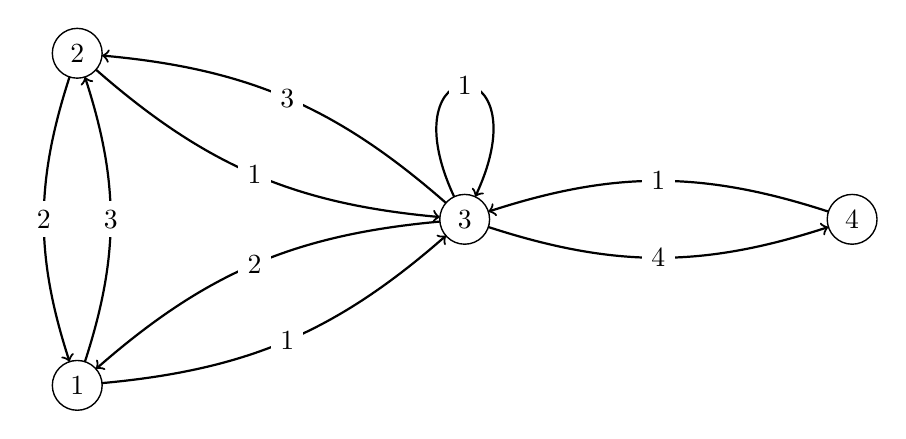
\begin{tikzpicture}[x=70,y=30]
          \Vertex{1}
          \NO[unit=4](1){2}
          \SOEA[unit=2](2){3}
          \EA[unit=2](3){4}
          \tikzset{EdgeStyle/.style = {->}}
          \tikzset{LoopStyle/.style = {->}}
          \tikzset{EdgeStyle/.append style = {bend right=18}}
          \only<1-2>{
            \Edge[label=1](1)(3)
            \Edge[label=3](1)(2)
            \Edge[label=2](2)(1)
            \Edge[label=1](2)(3)
            \Edge[label=2](3)(1)
            \Edge[label=3](3)(2)
            \Edge[label=4](3)(4)
            \draw[thick,->] (3) to [out=115,in=65,looseness=20] node [midway, fill=white] {1} (3);
            \Edge[label=1](4)(3)
          }
        \end{tikzpicture}
      \end{center}
      \uncover<2->{
        \[ u \to_\sigma v \qquad \norm{A_{\sigma}x}_v \leq \gamma \norm{x}_u. \]
      }
    }
  \end{frame}
  \begin{frame}{Is it enough ? \only<2>{\textcolor{green}{YES}}}
    \only<2>{
      \begin{block}{[Philippe et al. 2015]}
        For any $\epsilon > 0$, there exists a set of norms $\{\, \norm{\cdot}_v : v \in \Nodes \,\}$
        such that
        \[ \norm{A_\sigma x}_{v} \leq (\cjsr + \epsilon) \norm{x}_{u} \]
        holds for all \arc{} $(u,v,\sigma) \in \Arcs$.
      \end{block}
    }
  \end{frame}
  \begin{frame}{Why norms ?}
    \begin{itemize}
      \item Homogeneous,
      \item Positive,
      \item \only<1>{Convex} \only<2>{\sout{Convex} not needed}
    \end{itemize}
  \end{frame}
  \begin{frame}{Homogeneous positive polynomial}
    \begin{center}
      \includegraphics[trim=0cm 0cm 0cm .6cm, clip, height=.8\textheight]{polynomial.png}
    \end{center}
    \[ (x_1^2-x_2^2)^2 + \varepsilon(x_1^2+x_2^2)^2 \]
  \end{frame}
  \begin{frame}{Sum of Squares relaxation [Parrilo and Jadbabaie 2008]}
    \begin{block}{Barvinok's theorem}
      $\forall \norm{\cdot}$, $\exists p(x)$ SOS degree $2d$ such that
      \[ p(x)^{\frac{1}{2d}} \leq \norm{x} \leq {n+d-1 \choose d}^{\frac{1}{2d}}p(x)^{\frac{1}{2d}}. \]
    \end{block}
    \[ \norm{A_{\sigma}x}_v \leq \gamma \norm{x}_u \to p_v(A_\sigma x) \leq \gamma^{2d} {n+d-1 \choose d} p_u(x) \]
    \uncover<2>{
      \begin{block}{More tricky}
        \[ \gamma^{2d} {n+d-1 \choose d} p_u(x) - p_v(A_\sigma x) \text{ is SOS ?} \]
      \end{block}
    }
  \end{frame}
  \begin{frame}{Lyapunov functions}
    \Wider{
      \begin{center}
        \tabulinesep=0.5mm
        \begin{tabu}{{X[.7,c,m]X[c,m]X[c,m]X[c,m]X[c,m]}}
          & Node 1 & Node 2 & Node 3 & Node 4\\
          \PrimalFig{2}{1}
          \PrimalFig{4}{2}
          \PrimalFig{12}{6}
        \end{tabu}
      \end{center}
    }
  \end{frame}
  \begin{frame}{SOS Program}
    \begin{align*}
      \inf \gamma\\
      p_v(x) & \text{ is SOS} & \forall v \in \Nodes\\
      \gamma^{2d} p_u(x) - p_v(A_\sigma x) & \text{ is SOS} & \forall (u, v, \sigma) \in \Arcs.
    \end{align*}
  \end{frame}
  \begin{frame}{Pseudo-measure}
    \[
      \la \pE, p(x) \ra = \pE[p(x)] = \int_{\mathbb{S}^{n-1}} p(x) \dif \pmu \geq 0.
    \]
    $\forall p(x)$ SOS.
  \end{frame}
  \begin{frame}{Dual constraint: More flow in than out}
    \Wider{\begin{align*}
      \sum_{(u,v,\sigma) \in E} \pE_{uv\sigma}[p(A_\sigma x)] & \geq \gamma^{2d}\sum_{(v,w,\sigma) \in \Arcs} \pE_{vw\sigma}[p(x)], \qquad \forall v \in \Nodes, p(x) \text{ SOS},
    \end{align*}
    \begin{center}
      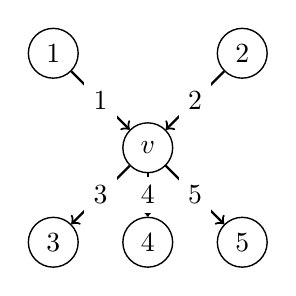
\begin{tikzpicture}
        \SetGraphUnit{1.2}
        \GraphInit[vstyle=Dijkstra]
        \SetUpEdge[style={->}]
        \Vertex[L=$v$]{0}
        \NOWE[L=$1$](0){4};
        \NOEA[L=$2$](0){5};
        \SOWE[L=$3$](0){10};
        \SO[L=$4$](0){11};
        \SOEA[L=$5$](0){12};
        \Edge[label=$1$](4)(0);
        \Edge[label=$2$](5)(0);
        \Edge[label=$3$](0)(10);
        \Edge[label=$4$](0)(11);
        \Edge[label=$5$](0)(12);
      \end{tikzpicture}
    \end{center}
    \begin{align*}
      \pE_{1v1}[p(A_1 x)] + \pE_{2v2}[p(A_2 x)] & \geq \gamma^{2d}(\pE_{v33}[p(x)] + \pE_{v44}[p(x)] + \pE_{v55}[p(x)]),
    \end{align*}
  }
  \end{frame}
  \section{Generating high growth sequences}
  \begin{frame}{Building a high growth sequence}
    \Wider{\[ \sum_{(u,v,\sigma) \in E} \pE_{uv\sigma}[p(A_\sigma x)] \geq \gamma^{2d}\sum_{(v,w,\sigma) \in \Arcs} \pE_{vw\sigma}[p(x)], \qquad \forall v \in \Nodes, p(x) \text{ SOS}, \]
    \begin{center}
      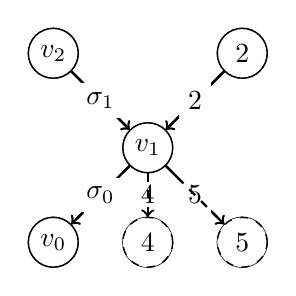
\begin{tikzpicture}
        \SetGraphUnit{1.2}
        \GraphInit[vstyle=Dijkstra]
        \SetUpEdge[style={->}]
        \uncover<1,2>{\Vertex[L=$v$]{0}}
        \uncover<3->{\Vertex[L=$v_1$]{0}}
        \uncover<1,2,3>{\NOWE[L=$1$](0){4};}
        \uncover<4>{\NOWE[L=$v_2$](0){4};}
        \uncover<1-3>{\NOEA[L=$2$](0){5};}
        \uncover<1,2>{
          \SOWE[L=$3$](0){10};
          \SO[L=$4$](0){11};
          \SOEA[L=$5$](0){12};
        }
        \uncover<3->{
          \SOWE[L=$v_0$](0){10};
          \tikzset{VertexStyle/.append style = {dashed}}
          \SO[L=$4$](0){11};
          \SOEA[L=$5$](0){12};
        }
        \uncover<4>{\NOEA[L=$2$](0){5};}
        \uncover<1-3>{\Edge[label=$1$](4)(0);}
        \uncover<4>{\Edge[label=$\sigma_1$](4)(0);}
        \uncover<1-3>{\Edge[label=$2$](5)(0);}
        \uncover<1,2>{
          \Edge[label=$3$](0)(10);
          \Edge[label=$4$](0)(11);
          \Edge[label=$5$](0)(12);
        }
        \uncover<3->{
          \tikzset{EdgeStyle/.append style = {dashed}}
          \Edge[label=$\sigma_0$](0)(10);
          \Edge(0)(11);
          \Edge(0)(12);
        }
        \uncover<4>{\Edge[label=$2$](5)(0);}
      \end{tikzpicture}
    \end{center}
    \begin{align*}
      \uncover<2->{\pE_{1v1}[p(A_1 x)] + \pE_{2v2}[p(A_2 x)] & \geq \gamma^{2d}(\pE_{v33}[p(x)] + \pE_{v44}[p(x)] + \pE_{v55}[p(x)]),\\}
      \uncover<3->{\pE_{1v_11}[p(A_1 x)] + \pE_{2v_12}[p(A_2 x)] & \geq \gamma^{2d}\pE_{v_1v_0\sigma_0}[p(x)],\\}
      \uncover<4>{\pE_{v_2v_1\sigma_1}[p(A_1 x)] & \geq \frac{1}{2} \gamma^{2d}\pE_{v_1v_0\sigma_0}[p(x)].}
    \end{align*}
  }
  \end{frame}
  \begin{frame}{Choice of polynomial}
    $p_0(x)$ random.

    \[ p_{k+1}(x) = p_{k}(A_{\sigma_k}x) = p_0(A_{\sigma_1} \cdots A_{\sigma_k} x) \]

    \begin{center}
      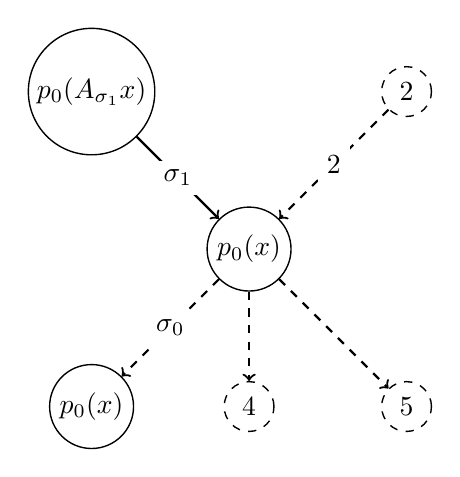
\begin{tikzpicture}
        \SetGraphUnit{2}
        \GraphInit[vstyle=Dijkstra]
        \SetUpEdge[style={->}]
        \Vertex[L=$p_0(x)$]{0}
        \NOWE[L=$p_0(A_{\sigma_1} x)$](0){4};
        \SOWE[L=$p_0(x)$](0){10};
        \tikzset{VertexStyle/.append style = {dashed}}
        \SO[L=$4$](0){11};
        \SOEA[L=$5$](0){12};
        \NOEA[L=$2$](0){5};
        \Edge[label=$\sigma_1$](4)(0);
        \tikzset{EdgeStyle/.append style = {dashed}}
        \Edge[label=$\sigma_0$](0)(10);
        \Edge(0)(11);
        \Edge(0)(12);
        \Edge[label=$2$](5)(0);
      \end{tikzpicture}
    \end{center}

  \end{frame}
  \begin{frame}{Guarantee on sequence produced}
    Let
    \[
      \theta_k \triangleq \pE_{v_{k+1}v_k\sigma_k}[p_{0}(A_{\sigma_1} \cdots A_{\sigma_k}x)].
    \]
    We have
    \[ \theta_{k} \geq \frac{\gamma^{2d}}{\din(v_k)} \theta_{k-1}. \]

    \uncover<2>{
      \hfill
      \[ \frac{\gamma}{\norm{\Adj^\Tr}_\infty^{\frac{1}{2d}}} \leq \lim_{k \to \infty} \norm{A_{\sigma_1} \cdots A_{\sigma_k}}^{\frac{1}{k}}. \]
    }
  \end{frame}
  \begin{frame}{Let's try it}
    \begin{center}
      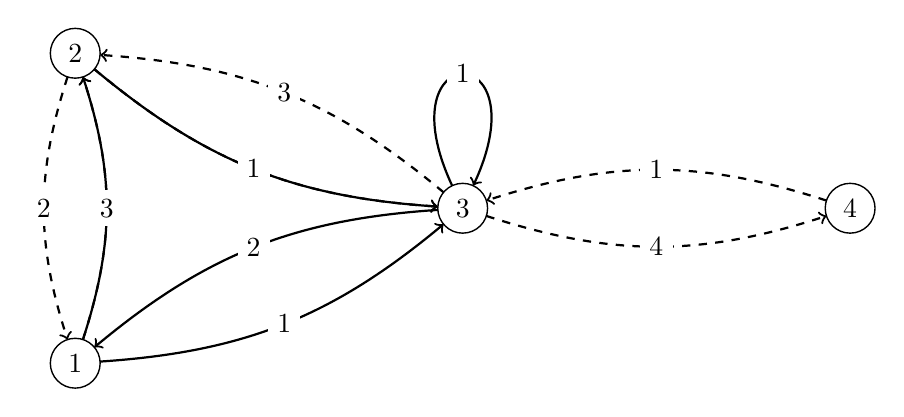
\begin{tikzpicture}[x=70,y=28]
        \Vertex{1}
        \NO[unit=4](1){2}
        \SOEA[unit=2](2){3}
        \EA[unit=2](3){4}
        \tikzset{EdgeStyle/.style = {->}}
        \tikzset{LoopStyle/.style = {->}}
        \tikzset{EdgeStyle/.append style = {bend right=18}}
        \Edge[label=1](1)(3)
        \Edge[label=2](3)(1)
        \draw[thick,->] (3) to [out=115,in=65,looseness=20] node [midway, fill=white] {1} (3);
        \uncover<2>{
          \Edge[label=3](1)(2)
          \Edge[label=1](2)(3)
        }
        \uncover<1>{
          \tikzset{EdgeStyle/.append style = {dashed}}
          \Edge[label=3](1)(2)
          \Edge[label=1](2)(3)
        }
        \tikzset{EdgeStyle/.append style = {dashed}}
        \Edge[label=2](2)(1)
        \Edge[label=3](3)(2)
        \Edge[label=4](3)(4)
        \Edge[label=1](4)(3)
      \end{tikzpicture}
      \hspace{1cm}
      \only<1>{
        $2d = 2$
        \[ 3 \to_2 1 \to_1 3 \to_2 1 \to_3 1 \to_1 3 \to_1 3 \to_1 3 \to_1 3 \to_1 3 \]
        $0.97\textcolor{red}{289}$
      }
      \only<2>{
        $2d = 12$
        \[ 3 \to_2 1 \to_1 3 \to_2 1 \to_3 2 \to_1 3 \to_1 3 \to_1 3 \to_1 3 \]
        $0.97\textcolor{green}{482}$
      }
    \end{center}
  \end{frame}
  \begin{frame}{Improvement}
    \only<1>{
      \begin{center}
      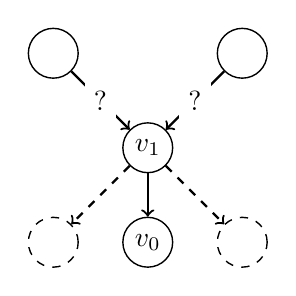
\begin{tikzpicture}
        \SetGraphUnit{1.2}
        \GraphInit[vstyle=Dijkstra]
        \SetVertexNoLabel
        \SetUpEdge[style={->}]
        \Vertex[NoLabel=false,L=$v_1$]{0}
        \NOWE(0){4};
        \NOEA(0){5};
        \SO[NoLabel=false,L=$v_0$](0){11};
        \tikzset{VertexStyle/.append style = {dashed}}
        \SOWE(0){10};
        \SOEA(0){12};
        \Edge[label=?](4)(0);
        \Edge[label=?](5)(0);
        \Edge(0)(11);
        \tikzset{EdgeStyle/.append style = {dashed}}
        \Edge(0)(10);
        \Edge(0)(12);
      \end{tikzpicture}
      \end{center}
    }
    \only<2>{
      \begin{center}
      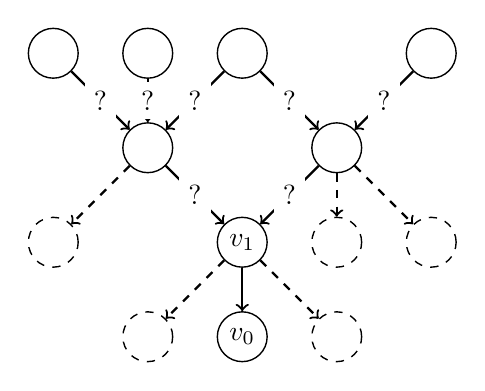
\begin{tikzpicture}
        \SetGraphUnit{1.2}
        \GraphInit[vstyle=Dijkstra]
        \SetVertexNoLabel
        \SetUpEdge[style={->}]
        \Vertex[NoLabel=false,L=$v_1$]{0}
        \NOWE(0){4};
        \NOEA(0){5};
        \NOWE(4){6};
        \NO  (4){7};
        \NOEA(4){8};
        \NOEA(5){9};
        \SO[NoLabel=false,L=$v_0$](0){11};
        \tikzset{VertexStyle/.append style = {dashed}}
        \SOWE(4){1};
        \EA(0){2};
        \EA(2){3};
        \SOWE(0){10};
        \SOEA(0){12};
        \Edge[label=?](6)(4);
        \Edge[label=?](7)(4);
        \Edge[label=?](8)(4);
        \Edge[label=?](8)(5);
        \Edge[label=?](9)(5);
        \Edge[label=?](4)(0);
        \Edge[label=?](5)(0);
        \Edge(0)(11);
        \tikzset{EdgeStyle/.append style = {dashed}}
        \Edge(4)(1);
        \Edge(5)(2);
        \Edge(5)(3);
        \Edge(0)(10);
        \Edge(0)(12);
      \end{tikzpicture}
      \end{center}
    }
  \end{frame}
  \begin{frame}{Improved guarantee}
    With horizon $l$:
    \[ \frac{\gamma}{\norm{[\Adj^\Tr]^l}_\infty^{\frac{1}{2dl}}} \leq \lim_{k \to \infty} \norm{A_{\sigma_1} \cdots A_{\sigma_k}}_2^{\frac{1}{k}}. \]
  \end{frame}
  \begin{frame}{Let's try it}
    \begin{center}
      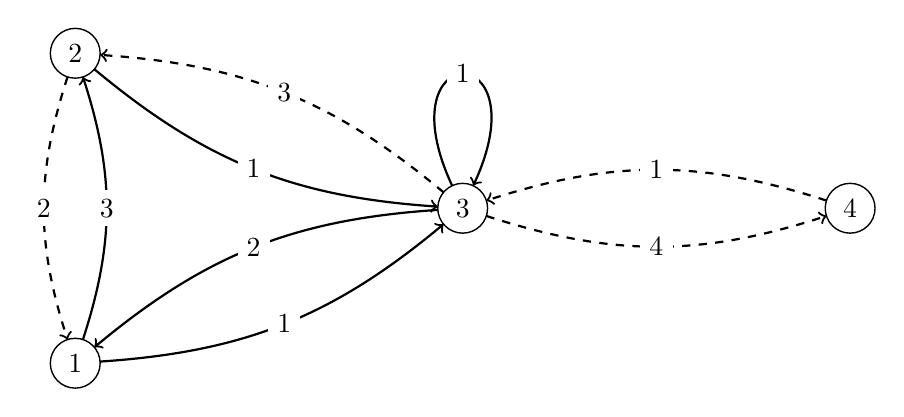
\begin{tikzpicture}[x=70,y=28]
        \Vertex{1}
        \NO[unit=4](1){2}
        \SOEA[unit=2](2){3}
        \EA[unit=2](3){4}
        \tikzset{EdgeStyle/.style = {->}}
        \tikzset{LoopStyle/.style = {->}}
        \tikzset{EdgeStyle/.append style = {bend right=18}}
        \Edge[label=1](1)(3)
        \Edge[label=2](3)(1)
        \draw[thick,->] (3) to [out=115,in=65,looseness=20] node [midway, fill=white] {1} (3);
        \Edge[label=3](1)(2)
        \Edge[label=1](2)(3)
        \tikzset{EdgeStyle/.append style = {dashed}}
        \Edge[label=2](2)(1)
        \Edge[label=3](3)(2)
        \Edge[label=4](3)(4)
        \Edge[label=1](4)(3)
      \end{tikzpicture}
      \hspace{1cm}
      $2d = 2, l = 3$
      \[ 3 \to_2 1 \to_1 3 \to_2 1 \to_3 2 \to_1 3 \to_1 3 \to_1 3 \to_1 3 \]
      $0.97\textcolor{green}{482}$
    \end{center}
  \end{frame}
  \subsection{Improved guarantee}
  \begin{frame}{Guarantee for the upper bound}
    As $l \to \infty$,
    \[ \rho(\Adj)^{-\frac{1}{2d}}\jsrsos \leq \lim_{k \to \infty} \norm{A_{\sigma_1} \cdots A_{\sigma_k}}^{\frac{1}{k}} \leq \cjsr \leq \jsrsos. \]


    Improving the lower bound:
    \begin{itemize}
      \item Use $\Adj(G')$ where edges of 0 dual variable are removed.
      \item Find lower bound in an high growth rate sequence produced.
    \end{itemize}
  \end{frame}
  \section{Conclusion}
  \begin{frame}{Conclusion}
    \begin{block}{Results}
      \begin{itemize}
        \item Algorithm producing sequence of growth rate asymptotically close to $\cjsr$.
        \item Guarantee on the ``closeness'' depending on $d$ and $\rho(\Adj)$.
        \item Provides improved lower bounds.
      \end{itemize}
    \end{block}
    \begin{block}{Open questions}
      \begin{itemize}
        \item Can we improve guarantee, e.g. using $n$ ?
        \item Is the sequence always periodic for a fixed $d$ ? Can we bound the period ?
      \end{itemize}
    \end{block}
  \end{frame}
\end{document}
